
Smartphone inertial sensors are used for driving analytics. 
The IMU accelerometer measures 3D acceleration 
\footnote{Depending on context, acceleration refers to either the 
rate of change of velocity per unit of time or the driving behavior
when the driver press the gas pedal.} 
changes and can be used to detect accelerations and brakes. 
The IMU gyroscope measures 3D angular change and can be used
to detect steering motions such as turns and lane changes.
Existing driving analytics approaches \cite{wang2013sensing,hansenspeed,chen2015invisible} 
assume ideal scenarios, i.e., 
the car is moving on flat road and  
the smartphone is stably mounted
with fixed relative orientation to the car. 


In trying to relax such assumptions, 
we found that the accuracy of inertial sensors, 
especially the accelerometer, are sensitive to road conditions, 
orientation changes and mounting stability (as a result of human interactions). 
We start with an example trip to illustrate the 
\emph{acceleration over/under estimation} problem
due to slopes and the effects of gravitation.  
We show that existing coordinate alignment
method may cause \emph{coordinate misalignment}. 
Such problems cannot be easily fixed due to 
the low accuracy of inertial sensors. 
We also discuss unmanaged smartphone usage
cases and the impacts on driving analytics, 
i.e., relative orientation changes and the 
smartphone is not stably mounted. 

\subsection{Sensitive to Road Conditions}

\subsubsection{Acceleration Over/Under Estimation}


\begin{figure}[!tbp] \centering
    \begin{subfigure}[b]{\linewidth}
         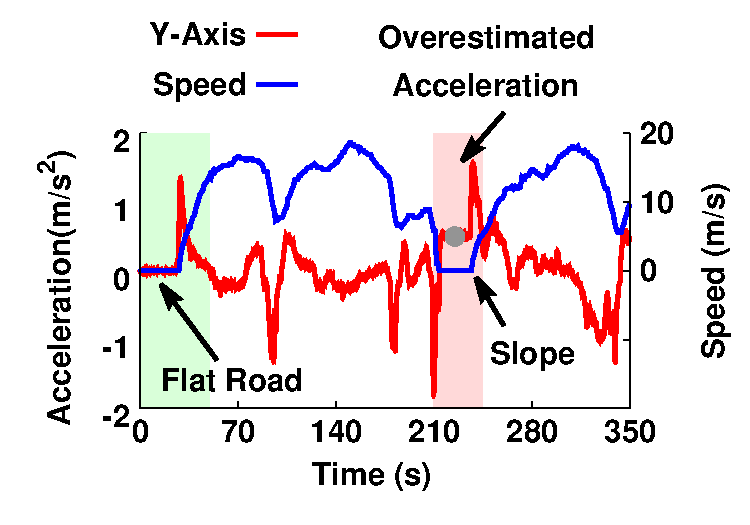
\includegraphics[width=3.3in,angle=0]{Figs/DriveSense/slopeaware/motivation.pdf}
         \vspace{-0.4cm}
         \caption{The accelerometer y-axis (along the car's heading direction) and OBD speed readings.}         
        \label{motivation:a}
    \end{subfigure} %

    \begin{subfigure}[b]{\linewidth}    
        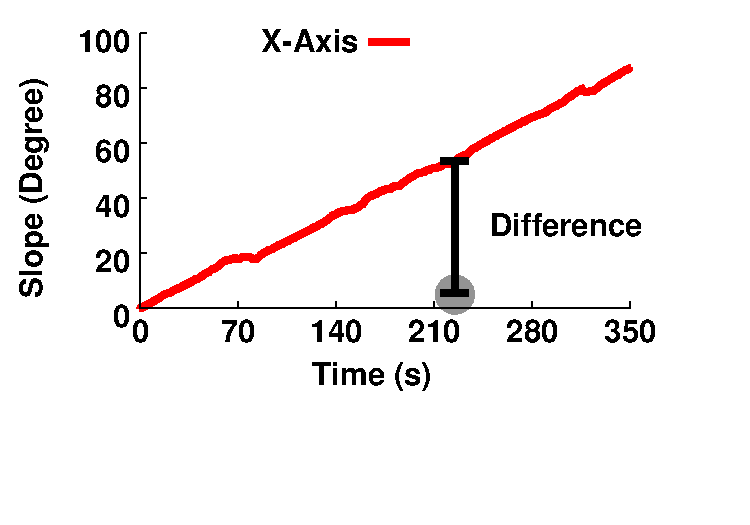
\includegraphics[width=3.3in,angle=0]{Figs/DriveSense/slopeaware/gyro_motivation.pdf}
        \vspace{-1.5cm}
        \caption{The accumulated gyroscope x-axis (tracking car's rotational speed when going upslope/downslope) readings.}
        \label{motivation:b}    
    \end{subfigure} 
\caption{Sensor and OBD data from the motivation example trip.}
\label{motivation}
\vspace{-0.2cm}
\end{figure}



We collect an example driving trip with various driving activities 
such as brakes and accelerations using a LG Nexus 5.
Before the trip, we park the car in a flat parking lot and fix
the smartphone with a frame mounted between the driver seat
and the passenger seat.
The coordinates of the phone are manually aligned (as precisely as we can) with the car. 
We use a customized Android application to record the sensor data and OBD speed data.
The sensor and OBD data traces of the trip are illustrated in Fig. \ref{motivation}.
As can be seen from the figure, the trip started on a flat road
and the speed was $0m/s$ with acceleration $0m/s^2$. 
At time $210s$, there is a stop as the OBD speed reading was $0m/s$ 
while the accelerometer reading is around $0.5m/s^2$ indicating
the car is accelerating. It is an overestimated acceleration
due to road slope.
This is because the y-axis of the accelerometer can sense the gravity. 
The gravitational force may have an incremental or decremental effect
on the estimation of vehicle motion parameters. 
For example, a misalignment of five degrees may cause $0.85m/s^2$ 
acceleration estimation error.
For reference, the \emph{Snapshot Program} \cite{snapshot} records a hard brake if the deceleration is around $3m/s^2$.
Therefore, we conclude that \emph{road slopes and associated gravitational effect
cause acceleration over/under estimation}. 


\subsubsection{Accumulated Gyroscope Errors}

The gyroscope can be used to track three-dimensional angular changes
and is an ideal input for slope estimation. 
However, it is known to suffer accumulated errors \cite{zhou2014use}. 
As illustrate in Fig. \ref{motivation}, 
we observe similar error accumulation in our motivation experiment. 
The dark dot is the slope gradient calculated by the accelerometer.
The curve of gyroscope measures the accumulated angular changes  
when the car was driving upslope/downslope.
Intuitively, the accumulated angular change of gyroscope can be used to 
estimate the slope gradients.
Clearly, the accumulated error is much higher than 
the actual accumulated slope gradients estimated by the accelerometer. 
We refer interested readers to \cite{chen2015invisible, zhou2014use},  
for detailed gyroscope three-dimensional readings 
and corresponding vehicle movement. 
Since we only focus on going upslope/downslope, we are interested in 
x-axis gyroscope readings of the car (or aligned smartphone) only.
There are several reasons why we see accumulated errors of gyroscope. 
The first one is the constant drifts, where the gyroscope reading is 
not zero in still due to limited hardware precision.
As the angular changes add up, the constant drifts accumulate correspondingly, 
which leads to a rough linear function between accumulated error and time.
The second one is the vibration of the vehicle, which accelerates
the drifts of the gyroscope readings.
Misalignment (caused by either manual alignment in our experiment 
or the coordinate alignment algorithm) between the car and the smartphone can also introduce accumulated errors. 
This is because the x-axis of the gyroscope can also sense car's steering angular change like turns and lane changes
when the smartphone is misaligned with the car.

\subsubsection{Coordinate Misalignment}

\begin{figure}[!htbp]
\begin{center}
  \vspace{-0.2cm}
  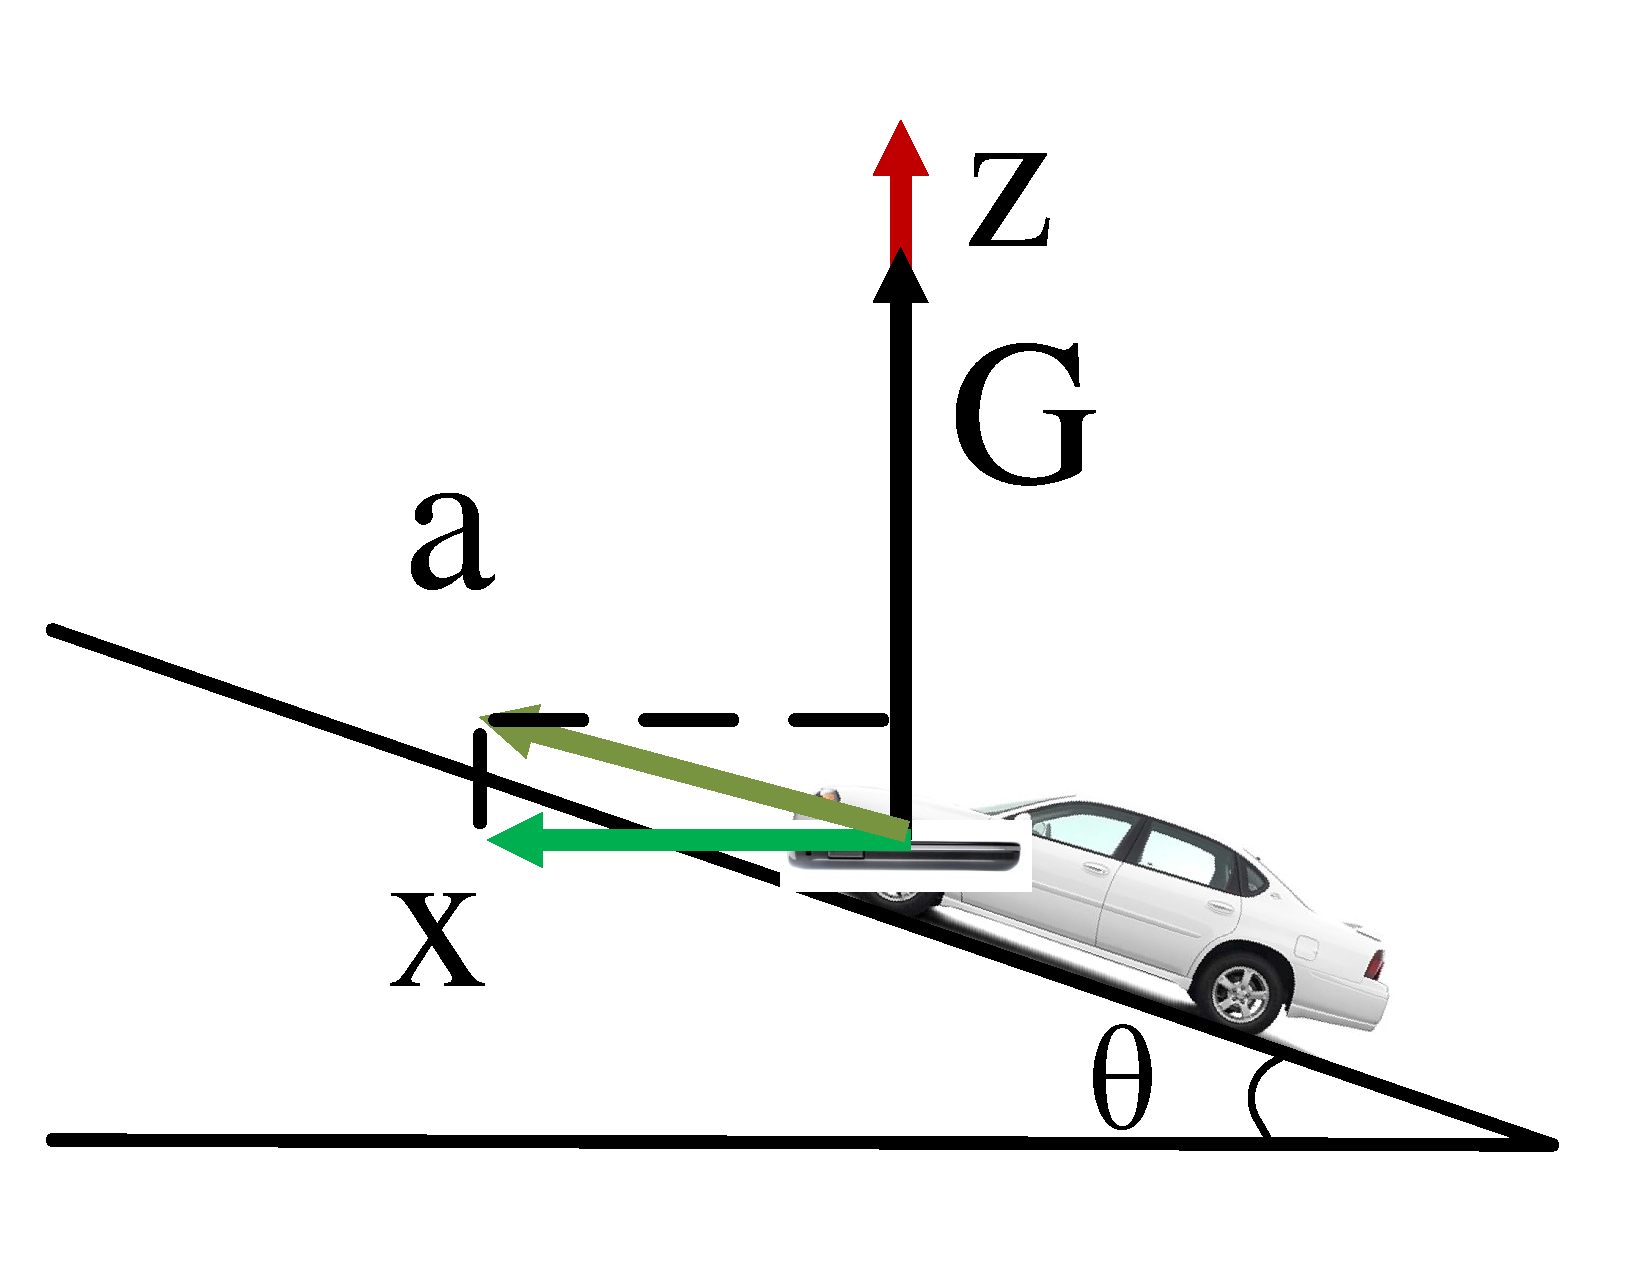
\includegraphics[width=2.6in, angle=0]{Figs/DriveSense/slopeaware/misalignment.pdf}
\vspace{-0.2cm}
\caption{Coordinate misalignment caused by road slopes.}
  \label{slopemisalignment}
\vspace{-0.4cm}
\end{center}
\end{figure}

Coordinate alignment is the process to align the
coordinates of the smartphone to those of the car 
\cite{hansenspeed, wang2013sensing, chen2015invisible}. 
We find that slopes cause misalignment
if the coordinate alignment is conducted on slope. 
Coordinate misalignment refers to the case when the aligned coordinates of 
the smartphone is not perfectly aligned with the coordinates of the car. 
Since the accelerometer can sense gravity, a misalignment
may also cause acceleration over/under estimation problem. 
As illustrated in Fig. \ref{slopemisalignment}, 
the car is moving upslope while the coordinate alignment algorithm
assumes the car is moving on flat road, 
which leads to the intersection angle $\theta$ between
aligned coordinates of the smartphone and the coordinates
of the car. 
Such misalignment may cause acceleration over/under estimation
when the driver is driving on flat road. 


\subsection{Sensitive to Human Interactions}


Human interactions may change the 
relative orientation and mounting stability of the smartphone, 
which degrade the usability and accuracy
of inertial sensors. 
Relative orientation change refers to the
orientation change of the smartphone independent of
the movement of the car. 
Imaging a passenger pick up the phone from pocket
and answer a phone call, 
the movement of the smartphone is the addition of 
the movement caused by human interactions and vehicle movements. 
Mounting stability refers to the degree of fixation of the smartphone, 
i.e., the mounting stability when the smartphone is fixed in car mount
it higher than the case when the smartphone is put in the pocket. 


The relative orientation change causes the sensor
readings are too noisy to be used.
Suppose the smartphone is rotated horizontally 
180 degree, then the output of accleleromter 
is completely reversed, i.e., the smartphone
detects brake when the car is accelerating. 
To eliminate such errors, 
the rotation matrix should be
re-estimated for accurate output. 
Coordinate alignment is an expensive process, 
which we will discuss in details in later sections, 
and frequent coordinate alignment may lead to 
gray period where the inertial sensors
cannot used for driving analytics. 



Mounting stability is also an important factor when 
conducting driving analytics by using inertial sensors. 
When the user puts
the smartphone in the pocket,
the vibration of smartphone may add extra noises.
We advocate the use of a metric to quantify mounting stability
and understand the sensor accuracy under
various stability levels. 


